% Created by tikzDevice version 0.12.6 on 2026-08-08 12:11:48
% !TEX encoding = UTF-8 Unicode
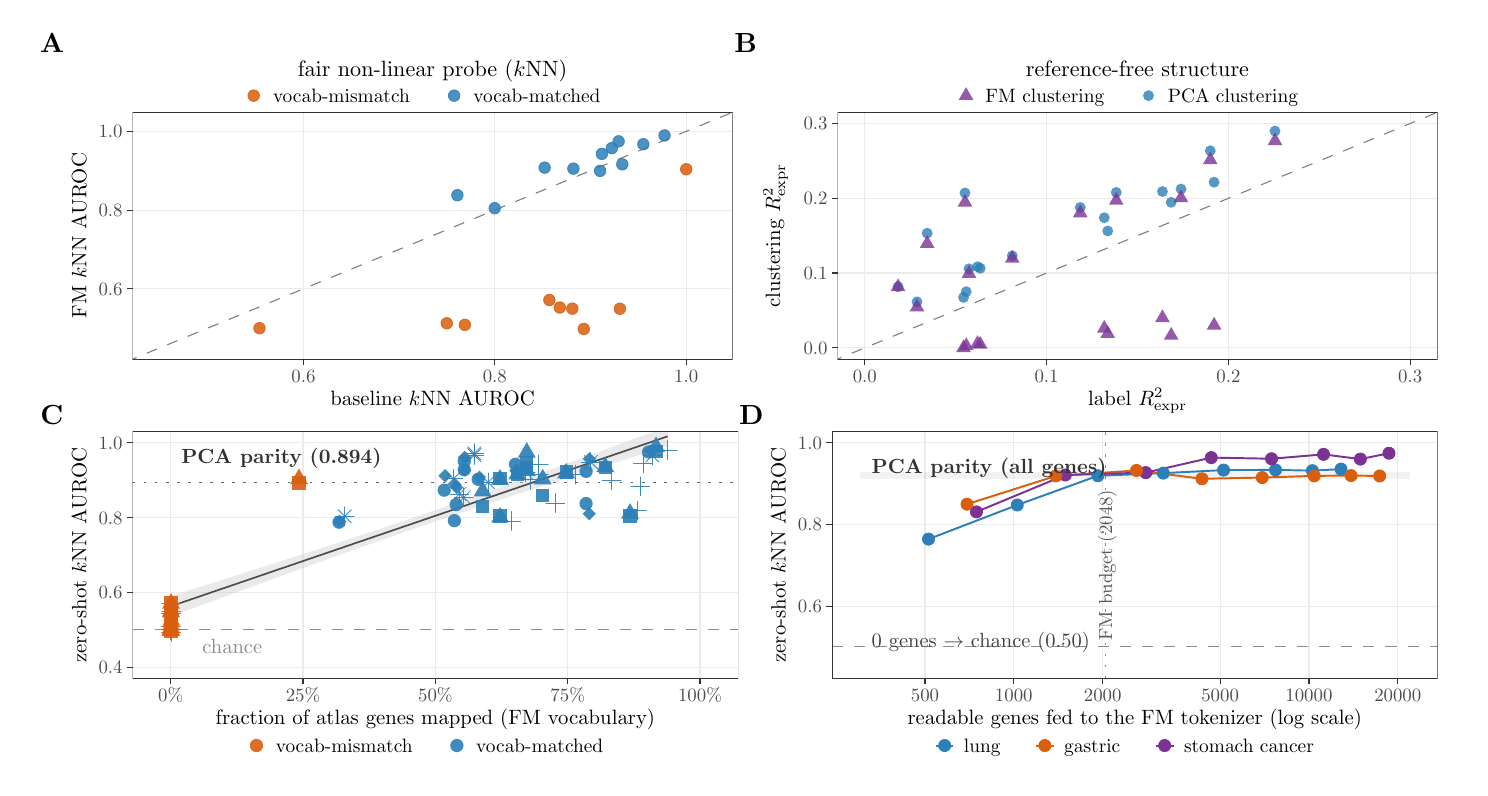
\begin{tikzpicture}[x=1pt,y=1pt]
\definecolor{fillColor}{RGB}{255,255,255}
\path[use as bounding box,fill=fillColor,fill opacity=0.00] (0,0) rectangle (517.45,267.40);
\begin{scope}
\path[clip] (  0.00,  0.00) rectangle (517.45,267.40);
\definecolor{drawColor}{RGB}{255,255,255}
\definecolor{fillColor}{RGB}{255,255,255}

\path[draw=drawColor,line width= 0.4pt,line join=round,line cap=round,fill=fillColor] (  0.00,  0.00) rectangle (517.45,267.40);
\end{scope}
\begin{scope}
\path[clip] (  8.00,127.42) rectangle (258.73,261.40);
\definecolor{drawColor}{RGB}{255,255,255}
\definecolor{fillColor}{RGB}{255,255,255}

\path[draw=drawColor,line width= 0.4pt,line join=round,line cap=round,fill=fillColor] (  8.00,127.42) rectangle (258.73,261.40);
\end{scope}
\begin{scope}
\path[clip] (258.73,127.42) rectangle (513.45,261.40);
\definecolor{drawColor}{RGB}{255,255,255}
\definecolor{fillColor}{RGB}{255,255,255}

\path[draw=drawColor,line width= 0.4pt,line join=round,line cap=round,fill=fillColor] (258.73,127.42) rectangle (513.45,261.40);
\end{scope}
\begin{scope}
\path[clip] ( 37.91,147.65) rectangle (254.73,236.83);
\definecolor{fillColor}{RGB}{255,255,255}

\path[fill=fillColor] ( 37.91,147.65) rectangle (254.73,236.83);
\definecolor{drawColor}{gray}{0.92}

\path[draw=drawColor,line width= 0.4pt,line join=round] ( 37.91,173.04) --
	(254.73,173.04);

\path[draw=drawColor,line width= 0.4pt,line join=round] ( 37.91,201.49) --
	(254.73,201.49);

\path[draw=drawColor,line width= 0.4pt,line join=round] ( 37.91,229.94) --
	(254.73,229.94);

\path[draw=drawColor,line width= 0.4pt,line join=round] ( 99.64,147.65) --
	( 99.64,236.83);

\path[draw=drawColor,line width= 0.4pt,line join=round] (168.80,147.65) --
	(168.80,236.83);

\path[draw=drawColor,line width= 0.4pt,line join=round] (237.96,147.65) --
	(237.96,236.83);
\definecolor{drawColor}{gray}{0.50}

\path[draw=drawColor,line width= 0.4pt,dash pattern=on 4pt off 4pt ,line join=round] (-178.91, 58.46) -- (471.54,326.02);
\definecolor{drawColor}{RGB}{44,127,184}
\definecolor{fillColor}{RGB}{44,127,184}

\path[draw=drawColor,draw opacity=0.85,line width= 0.3pt,line join=round,line cap=round,fill=fillColor,fill opacity=0.85] (211.09,223.86) circle (  2.08);

\path[draw=drawColor,draw opacity=0.85,line width= 0.3pt,line join=round,line cap=round,fill=fillColor,fill opacity=0.85] (155.27,206.85) circle (  2.08);
\definecolor{drawColor}{RGB}{217,95,14}
\definecolor{fillColor}{RGB}{217,95,14}

\path[draw=drawColor,draw opacity=0.85,line width= 0.3pt,line join=round,line cap=round,fill=fillColor,fill opacity=0.85] (196.81,165.87) circle (  2.08);
\definecolor{drawColor}{RGB}{44,127,184}
\definecolor{fillColor}{RGB}{44,127,184}

\path[draw=drawColor,draw opacity=0.85,line width= 0.3pt,line join=round,line cap=round,fill=fillColor,fill opacity=0.85] (168.76,202.17) circle (  2.08);

\path[draw=drawColor,draw opacity=0.85,line width= 0.3pt,line join=round,line cap=round,fill=fillColor,fill opacity=0.85] (197.19,216.46) circle (  2.08);
\definecolor{drawColor}{RGB}{217,95,14}
\definecolor{fillColor}{RGB}{217,95,14}

\path[draw=drawColor,draw opacity=0.85,line width= 0.3pt,line join=round,line cap=round,fill=fillColor,fill opacity=0.85] (188.51,169.00) circle (  2.08);
\definecolor{drawColor}{RGB}{44,127,184}
\definecolor{fillColor}{RGB}{44,127,184}

\path[draw=drawColor,draw opacity=0.85,line width= 0.3pt,line join=round,line cap=round,fill=fillColor,fill opacity=0.85] (206.83,215.65) circle (  2.08);
\definecolor{drawColor}{RGB}{217,95,14}
\definecolor{fillColor}{RGB}{217,95,14}

\path[draw=drawColor,draw opacity=0.85,line width= 0.3pt,line join=round,line cap=round,fill=fillColor,fill opacity=0.85] (192.28,166.27) circle (  2.08);
\definecolor{drawColor}{RGB}{44,127,184}
\definecolor{fillColor}{RGB}{44,127,184}

\path[draw=drawColor,draw opacity=0.85,line width= 0.3pt,line join=round,line cap=round,fill=fillColor,fill opacity=0.85] (214.86,218.01) circle (  2.08);

\path[draw=drawColor,draw opacity=0.85,line width= 0.3pt,line join=round,line cap=round,fill=fillColor,fill opacity=0.85] (186.81,216.83) circle (  2.08);

\path[draw=drawColor,draw opacity=0.85,line width= 0.3pt,line join=round,line cap=round,fill=fillColor,fill opacity=0.85] (222.46,225.28) circle (  2.08);

\path[draw=drawColor,draw opacity=0.85,line width= 0.3pt,line join=round,line cap=round,fill=fillColor,fill opacity=0.85] (207.49,221.80) circle (  2.08);
\definecolor{drawColor}{RGB}{217,95,14}
\definecolor{fillColor}{RGB}{217,95,14}

\path[draw=drawColor,draw opacity=0.85,line width= 0.3pt,line join=round,line cap=round,fill=fillColor,fill opacity=0.85] (237.96,216.24) circle (  2.08);

\path[draw=drawColor,draw opacity=0.85,line width= 0.3pt,line join=round,line cap=round,fill=fillColor,fill opacity=0.85] ( 83.76,158.81) circle (  2.08);

\path[draw=drawColor,draw opacity=0.85,line width= 0.3pt,line join=round,line cap=round,fill=fillColor,fill opacity=0.85] (200.95,158.53) circle (  2.08);
\definecolor{drawColor}{RGB}{44,127,184}
\definecolor{fillColor}{RGB}{44,127,184}

\path[draw=drawColor,draw opacity=0.85,line width= 0.3pt,line join=round,line cap=round,fill=fillColor,fill opacity=0.85] (230.14,228.46) circle (  2.08);
\definecolor{drawColor}{RGB}{217,95,14}
\definecolor{fillColor}{RGB}{217,95,14}

\path[draw=drawColor,draw opacity=0.85,line width= 0.3pt,line join=round,line cap=round,fill=fillColor,fill opacity=0.85] (151.44,160.58) circle (  2.08);
\definecolor{drawColor}{RGB}{44,127,184}
\definecolor{fillColor}{RGB}{44,127,184}

\path[draw=drawColor,draw opacity=0.85,line width= 0.3pt,line join=round,line cap=round,fill=fillColor,fill opacity=0.85] (213.54,226.32) circle (  2.08);
\definecolor{drawColor}{RGB}{217,95,14}
\definecolor{fillColor}{RGB}{217,95,14}

\path[draw=drawColor,draw opacity=0.85,line width= 0.3pt,line join=round,line cap=round,fill=fillColor,fill opacity=0.85] (213.99,165.84) circle (  2.08);

\path[draw=drawColor,draw opacity=0.85,line width= 0.3pt,line join=round,line cap=round,fill=fillColor,fill opacity=0.85] (157.97,160.02) circle (  2.08);
\definecolor{drawColor}{gray}{0.20}

\path[draw=drawColor,line width= 0.4pt,line join=round,line cap=round] ( 37.91,147.65) rectangle (254.73,236.83);
\end{scope}
\begin{scope}
\path[clip] (  0.00,  0.00) rectangle (517.45,267.40);
\definecolor{drawColor}{gray}{0.30}

\node[text=drawColor,anchor=base east,inner sep=0pt, outer sep=0pt, scale=  0.68] at ( 34.31,170.69) {0.6};

\node[text=drawColor,anchor=base east,inner sep=0pt, outer sep=0pt, scale=  0.68] at ( 34.31,199.14) {0.8};

\node[text=drawColor,anchor=base east,inner sep=0pt, outer sep=0pt, scale=  0.68] at ( 34.31,227.59) {1.0};
\end{scope}
\begin{scope}
\path[clip] (  0.00,  0.00) rectangle (517.45,267.40);
\definecolor{drawColor}{gray}{0.20}

\path[draw=drawColor,line width= 0.4pt,line join=round] ( 35.91,173.04) --
	( 37.91,173.04);

\path[draw=drawColor,line width= 0.4pt,line join=round] ( 35.91,201.49) --
	( 37.91,201.49);

\path[draw=drawColor,line width= 0.4pt,line join=round] ( 35.91,229.94) --
	( 37.91,229.94);
\end{scope}
\begin{scope}
\path[clip] (  0.00,  0.00) rectangle (517.45,267.40);
\definecolor{drawColor}{gray}{0.20}

\path[draw=drawColor,line width= 0.4pt,line join=round] ( 99.64,145.65) --
	( 99.64,147.65);

\path[draw=drawColor,line width= 0.4pt,line join=round] (168.80,145.65) --
	(168.80,147.65);

\path[draw=drawColor,line width= 0.4pt,line join=round] (237.96,145.65) --
	(237.96,147.65);
\end{scope}
\begin{scope}
\path[clip] (  0.00,  0.00) rectangle (517.45,267.40);
\definecolor{drawColor}{gray}{0.30}

\node[text=drawColor,anchor=base,inner sep=0pt, outer sep=0pt, scale=  0.68] at ( 99.64,139.36) {0.6};

\node[text=drawColor,anchor=base,inner sep=0pt, outer sep=0pt, scale=  0.68] at (168.80,139.36) {0.8};

\node[text=drawColor,anchor=base,inner sep=0pt, outer sep=0pt, scale=  0.68] at (237.96,139.36) {1.0};
\end{scope}
\begin{scope}
\path[clip] (  0.00,  0.00) rectangle (517.45,267.40);
\definecolor{drawColor}{RGB}{0,0,0}

\node[text=drawColor,anchor=base,inner sep=0pt, outer sep=0pt, scale=  0.75] at (146.32,130.88) {baseline $k$NN AUROC};
\end{scope}
\begin{scope}
\path[clip] (  0.00,  0.00) rectangle (517.45,267.40);
\definecolor{drawColor}{RGB}{0,0,0}

\node[text=drawColor,rotate= 90.00,anchor=base,inner sep=0pt, outer sep=0pt, scale=  0.75] at ( 21.17,192.24) {FM $k$NN AUROC};
\end{scope}
\begin{scope}
\path[clip] (  0.00,  0.00) rectangle (517.45,267.40);
\definecolor{fillColor}{RGB}{255,255,255}

\path[fill=fillColor] ( 76.67,238.83) rectangle (215.96,246.83);
\end{scope}
\begin{scope}
\path[clip] (  0.00,  0.00) rectangle (517.45,267.40);
\definecolor{fillColor}{RGB}{255,255,255}

\path[fill=fillColor] ( 77.67,238.83) rectangle ( 85.67,246.83);
\definecolor{drawColor}{RGB}{217,95,14}
\definecolor{fillColor}{RGB}{217,95,14}

\path[draw=drawColor,draw opacity=0.85,line width= 0.3pt,line join=round,line cap=round,fill=fillColor,fill opacity=0.85] ( 81.67,242.83) circle (  2.08);
\end{scope}
\begin{scope}
\path[clip] (  0.00,  0.00) rectangle (517.45,267.40);
\definecolor{fillColor}{RGB}{255,255,255}

\path[fill=fillColor] (150.09,238.83) rectangle (158.09,246.83);
\definecolor{drawColor}{RGB}{44,127,184}
\definecolor{fillColor}{RGB}{44,127,184}

\path[draw=drawColor,draw opacity=0.85,line width= 0.3pt,line join=round,line cap=round,fill=fillColor,fill opacity=0.85] (154.09,242.83) circle (  2.08);
\end{scope}
\begin{scope}
\path[clip] (  0.00,  0.00) rectangle (517.45,267.40);
\definecolor{drawColor}{RGB}{0,0,0}

\node[text=drawColor,anchor=base west,inner sep=0pt, outer sep=0pt, scale=  0.70] at ( 88.67,240.42) {vocab-mismatch};
\end{scope}
\begin{scope}
\path[clip] (  0.00,  0.00) rectangle (517.45,267.40);
\definecolor{drawColor}{RGB}{0,0,0}

\node[text=drawColor,anchor=base west,inner sep=0pt, outer sep=0pt, scale=  0.70] at (161.09,240.42) {vocab-matched};
\end{scope}
\begin{scope}
\path[clip] (  0.00,  0.00) rectangle (517.45,267.40);
\definecolor{drawColor}{RGB}{0,0,0}

\node[text=drawColor,anchor=base,inner sep=0pt, outer sep=0pt, scale=  0.80] at (146.32,249.89) {fair non-linear probe ($k$NN)};
\end{scope}
\begin{scope}
\path[clip] (  0.00,  0.00) rectangle (517.45,267.40);
\definecolor{drawColor}{RGB}{0,0,0}

\node[text=drawColor,anchor=base,inner sep=0pt, outer sep=0pt, scale=  1.00] at (  8.84,258.25) {\bfseries A};
\end{scope}
\begin{scope}
\path[clip] (292.64,147.65) rectangle (509.45,236.83);
\definecolor{fillColor}{RGB}{255,255,255}

\path[fill=fillColor] (292.64,147.65) rectangle (509.45,236.83);
\definecolor{drawColor}{gray}{0.92}

\path[draw=drawColor,line width= 0.4pt,line join=round] (292.64,151.70) --
	(509.45,151.70);

\path[draw=drawColor,line width= 0.4pt,line join=round] (292.64,178.73) --
	(509.45,178.73);

\path[draw=drawColor,line width= 0.4pt,line join=round] (292.64,205.75) --
	(509.45,205.75);

\path[draw=drawColor,line width= 0.4pt,line join=round] (292.64,232.78) --
	(509.45,232.78);

\path[draw=drawColor,line width= 0.4pt,line join=round] (302.49,147.65) --
	(302.49,236.83);

\path[draw=drawColor,line width= 0.4pt,line join=round] (368.19,147.65) --
	(368.19,236.83);

\path[draw=drawColor,line width= 0.4pt,line join=round] (433.90,147.65) --
	(433.90,236.83);

\path[draw=drawColor,line width= 0.4pt,line join=round] (499.60,147.65) --
	(499.60,236.83);
\definecolor{drawColor}{gray}{0.50}

\path[draw=drawColor,line width= 0.4pt,dash pattern=on 4pt off 4pt ,line join=round] ( 75.82, 58.46) -- (726.27,326.02);
\definecolor{fillColor}{RGB}{44,127,184}

\path[fill=fillColor,fill opacity=0.80] (355.78,184.97) circle (  1.97);

\path[fill=fillColor,fill opacity=0.80] (340.14,180.27) circle (  1.97);

\path[fill=fillColor,fill opacity=0.80] (390.27,193.94) circle (  1.97);

\path[fill=fillColor,fill opacity=0.80] (450.72,230.02) circle (  1.97);

\path[fill=fillColor,fill opacity=0.80] (321.35,168.32) circle (  1.97);

\path[fill=fillColor,fill opacity=0.80] (410.05,208.19) circle (  1.97);

\path[fill=fillColor,fill opacity=0.80] (380.35,202.43) circle (  1.97);

\path[fill=fillColor,fill opacity=0.80] (428.71,211.56) circle (  1.97);

\path[fill=fillColor,fill opacity=0.80] (338.69,207.67) circle (  1.97);

\path[fill=fillColor,fill opacity=0.80] (314.52,173.78) circle (  1.97);

\path[fill=fillColor,fill opacity=0.80] (427.33,222.92) circle (  1.97);

\path[fill=fillColor,fill opacity=0.80] (416.75,209.08) circle (  1.97);

\path[fill=fillColor,fill opacity=0.80] (413.20,204.29) circle (  1.97);

\path[fill=fillColor,fill opacity=0.80] (338.17,169.92) circle (  1.97);

\path[fill=fillColor,fill opacity=0.80] (339.15,172.00) circle (  1.97);

\path[fill=fillColor,fill opacity=0.80] (393.36,207.86) circle (  1.97);

\path[fill=fillColor,fill opacity=0.80] (344.21,180.46) circle (  1.97);

\path[fill=fillColor,fill opacity=0.80] (325.03,193.13) circle (  1.97);

\path[fill=fillColor,fill opacity=0.80] (389.02,198.73) circle (  1.97);

\path[fill=fillColor,fill opacity=0.80] (343.23,181.02) circle (  1.97);
\definecolor{fillColor}{RGB}{123,50,148}

\path[fill=fillColor,fill opacity=0.80] (355.78,187.09) --
	(358.43,182.49) --
	(353.12,182.49) --
	cycle;

\path[fill=fillColor,fill opacity=0.80] (340.14,181.58) --
	(342.80,176.98) --
	(337.48,176.98) --
	cycle;

\path[fill=fillColor,fill opacity=0.80] (390.27,159.90) --
	(392.93,155.30) --
	(387.61,155.30) --
	cycle;

\path[fill=fillColor,fill opacity=0.80] (450.72,229.55) --
	(453.37,224.95) --
	(448.06,224.95) --
	cycle;

\path[fill=fillColor,fill opacity=0.80] (321.35,169.50) --
	(324.00,164.90) --
	(318.69,164.90) --
	cycle;

\path[fill=fillColor,fill opacity=0.80] (410.05,165.60) --
	(412.70,161.00) --
	(407.39,161.00) --
	cycle;

\path[fill=fillColor,fill opacity=0.80] (380.35,203.47) --
	(383.00,198.87) --
	(377.69,198.87) --
	cycle;

\path[fill=fillColor,fill opacity=0.80] (428.71,162.93) --
	(431.36,158.33) --
	(426.05,158.33) --
	cycle;

\path[fill=fillColor,fill opacity=0.80] (338.69,207.36) --
	(341.35,202.76) --
	(336.04,202.76) --
	cycle;

\path[fill=fillColor,fill opacity=0.80] (314.52,176.79) --
	(317.17,172.19) --
	(311.86,172.19) --
	cycle;

\path[fill=fillColor,fill opacity=0.80] (427.33,222.66) --
	(429.98,218.06) --
	(424.67,218.06) --
	cycle;

\path[fill=fillColor,fill opacity=0.80] (416.75,208.93) --
	(419.40,204.33) --
	(414.09,204.33) --
	cycle;

\path[fill=fillColor,fill opacity=0.80] (413.20,159.25) --
	(415.86,154.65) --
	(410.54,154.65) --
	cycle;

\path[fill=fillColor,fill opacity=0.80] (338.17,154.77) --
	(340.82,150.17) --
	(335.51,150.17) --
	cycle;

\path[fill=fillColor,fill opacity=0.80] (339.15,155.52) --
	(341.81,150.92) --
	(336.50,150.92) --
	cycle;

\path[fill=fillColor,fill opacity=0.80] (393.36,208.04) --
	(396.01,203.44) --
	(390.70,203.44) --
	cycle;

\path[fill=fillColor,fill opacity=0.80] (344.21,156.01) --
	(346.87,151.41) --
	(341.56,151.41) --
	cycle;

\path[fill=fillColor,fill opacity=0.80] (325.03,192.47) --
	(327.68,187.87) --
	(322.37,187.87) --
	cycle;

\path[fill=fillColor,fill opacity=0.80] (389.02,161.79) --
	(391.68,157.19) --
	(386.37,157.19) --
	cycle;

\path[fill=fillColor,fill opacity=0.80] (343.23,156.28) --
	(345.88,151.68) --
	(340.57,151.68) --
	cycle;
\definecolor{drawColor}{gray}{0.20}

\path[draw=drawColor,line width= 0.4pt,line join=round,line cap=round] (292.64,147.65) rectangle (509.45,236.83);
\end{scope}
\begin{scope}
\path[clip] (  0.00,  0.00) rectangle (517.45,267.40);
\definecolor{drawColor}{gray}{0.30}

\node[text=drawColor,anchor=base east,inner sep=0pt, outer sep=0pt, scale=  0.68] at (289.04,149.36) {0.0};

\node[text=drawColor,anchor=base east,inner sep=0pt, outer sep=0pt, scale=  0.68] at (289.04,176.38) {0.1};

\node[text=drawColor,anchor=base east,inner sep=0pt, outer sep=0pt, scale=  0.68] at (289.04,203.41) {0.2};

\node[text=drawColor,anchor=base east,inner sep=0pt, outer sep=0pt, scale=  0.68] at (289.04,230.44) {0.3};
\end{scope}
\begin{scope}
\path[clip] (  0.00,  0.00) rectangle (517.45,267.40);
\definecolor{drawColor}{gray}{0.20}

\path[draw=drawColor,line width= 0.4pt,line join=round] (290.64,151.70) --
	(292.64,151.70);

\path[draw=drawColor,line width= 0.4pt,line join=round] (290.64,178.73) --
	(292.64,178.73);

\path[draw=drawColor,line width= 0.4pt,line join=round] (290.64,205.75) --
	(292.64,205.75);

\path[draw=drawColor,line width= 0.4pt,line join=round] (290.64,232.78) --
	(292.64,232.78);
\end{scope}
\begin{scope}
\path[clip] (  0.00,  0.00) rectangle (517.45,267.40);
\definecolor{drawColor}{gray}{0.20}

\path[draw=drawColor,line width= 0.4pt,line join=round] (302.49,145.65) --
	(302.49,147.65);

\path[draw=drawColor,line width= 0.4pt,line join=round] (368.19,145.65) --
	(368.19,147.65);

\path[draw=drawColor,line width= 0.4pt,line join=round] (433.90,145.65) --
	(433.90,147.65);

\path[draw=drawColor,line width= 0.4pt,line join=round] (499.60,145.65) --
	(499.60,147.65);
\end{scope}
\begin{scope}
\path[clip] (  0.00,  0.00) rectangle (517.45,267.40);
\definecolor{drawColor}{gray}{0.30}

\node[text=drawColor,anchor=base,inner sep=0pt, outer sep=0pt, scale=  0.68] at (302.49,139.36) {0.0};

\node[text=drawColor,anchor=base,inner sep=0pt, outer sep=0pt, scale=  0.68] at (368.19,139.36) {0.1};

\node[text=drawColor,anchor=base,inner sep=0pt, outer sep=0pt, scale=  0.68] at (433.90,139.36) {0.2};

\node[text=drawColor,anchor=base,inner sep=0pt, outer sep=0pt, scale=  0.68] at (499.60,139.36) {0.3};
\end{scope}
\begin{scope}
\path[clip] (  0.00,  0.00) rectangle (517.45,267.40);
\definecolor{drawColor}{RGB}{0,0,0}

\node[text=drawColor,anchor=base,inner sep=0pt, outer sep=0pt, scale=  0.75] at (401.04,130.88) {label $R^2_{\mathrm{expr}}$};
\end{scope}
\begin{scope}
\path[clip] (  0.00,  0.00) rectangle (517.45,267.40);
\definecolor{drawColor}{RGB}{0,0,0}

\node[text=drawColor,rotate= 90.00,anchor=base,inner sep=0pt, outer sep=0pt, scale=  0.75] at (271.89,192.24) {clustering $R^2_{\mathrm{expr}}$};
\end{scope}
\begin{scope}
\path[clip] (  0.00,  0.00) rectangle (517.45,267.40);
\definecolor{fillColor}{RGB}{255,255,255}

\path[fill=fillColor] (334.08,238.83) rectangle (468.01,246.83);
\end{scope}
\begin{scope}
\path[clip] (  0.00,  0.00) rectangle (517.45,267.40);
\definecolor{fillColor}{RGB}{255,255,255}

\path[fill=fillColor] (335.08,238.83) rectangle (343.08,246.83);
\definecolor{fillColor}{RGB}{123,50,148}

\path[fill=fillColor,fill opacity=0.80] (339.08,245.90) --
	(341.74,241.30) --
	(336.42,241.30) --
	cycle;
\end{scope}
\begin{scope}
\path[clip] (  0.00,  0.00) rectangle (517.45,267.40);
\definecolor{fillColor}{RGB}{255,255,255}

\path[fill=fillColor] (401.00,238.83) rectangle (409.00,246.83);
\definecolor{fillColor}{RGB}{44,127,184}

\path[fill=fillColor,fill opacity=0.80] (405.00,242.83) circle (  1.97);
\end{scope}
\begin{scope}
\path[clip] (  0.00,  0.00) rectangle (517.45,267.40);
\definecolor{drawColor}{RGB}{0,0,0}

\node[text=drawColor,anchor=base west,inner sep=0pt, outer sep=0pt, scale=  0.70] at (346.08,240.42) {FM clustering};
\end{scope}
\begin{scope}
\path[clip] (  0.00,  0.00) rectangle (517.45,267.40);
\definecolor{drawColor}{RGB}{0,0,0}

\node[text=drawColor,anchor=base west,inner sep=0pt, outer sep=0pt, scale=  0.70] at (412.00,240.42) {PCA clustering};
\end{scope}
\begin{scope}
\path[clip] (  0.00,  0.00) rectangle (517.45,267.40);
\definecolor{drawColor}{RGB}{0,0,0}

\node[text=drawColor,anchor=base,inner sep=0pt, outer sep=0pt, scale=  0.80] at (401.04,249.89) {reference-free structure};
\end{scope}
\begin{scope}
\path[clip] (  0.00,  0.00) rectangle (517.45,267.40);
\definecolor{drawColor}{RGB}{0,0,0}

\node[text=drawColor,anchor=base,inner sep=0pt, outer sep=0pt, scale=  1.00] at (259.44,258.25) {\bfseries B};
\end{scope}
\begin{scope}
\path[clip] (  8.00,  2.00) rectangle (260.73,127.42);
\definecolor{drawColor}{RGB}{255,255,255}
\definecolor{fillColor}{RGB}{255,255,255}

\path[draw=drawColor,line width= 0.4pt,line join=round,line cap=round,fill=fillColor] (  8.00,  2.00) rectangle (260.73,127.42);
\end{scope}
\begin{scope}
\path[clip] (260.73,  2.00) rectangle (513.45,127.42);
\definecolor{drawColor}{RGB}{255,255,255}
\definecolor{fillColor}{RGB}{255,255,255}

\path[draw=drawColor,line width= 0.4pt,line join=round,line cap=round,fill=fillColor] (260.73,  2.00) rectangle (513.45,127.42);
\end{scope}
\begin{scope}
\path[clip] ( 37.91, 32.23) rectangle (256.73,121.42);
\definecolor{fillColor}{RGB}{255,255,255}

\path[fill=fillColor] ( 37.91, 32.23) rectangle (256.73,121.42);
\definecolor{drawColor}{gray}{0.92}

\path[draw=drawColor,line width= 0.4pt,line join=round] ( 37.91, 36.28) --
	(256.73, 36.28);

\path[draw=drawColor,line width= 0.4pt,line join=round] ( 37.91, 63.31) --
	(256.73, 63.31);

\path[draw=drawColor,line width= 0.4pt,line join=round] ( 37.91, 90.34) --
	(256.73, 90.34);

\path[draw=drawColor,line width= 0.4pt,line join=round] ( 37.91,117.36) --
	(256.73,117.36);

\path[draw=drawColor,line width= 0.4pt,line join=round] ( 51.68, 32.23) --
	( 51.68,121.42);

\path[draw=drawColor,line width= 0.4pt,line join=round] ( 99.50, 32.23) --
	( 99.50,121.42);

\path[draw=drawColor,line width= 0.4pt,line join=round] (147.32, 32.23) --
	(147.32,121.42);

\path[draw=drawColor,line width= 0.4pt,line join=round] (195.14, 32.23) --
	(195.14,121.42);

\path[draw=drawColor,line width= 0.4pt,line join=round] (242.95, 32.23) --
	(242.95,121.42);
\definecolor{drawColor}{gray}{0.55}

\path[draw=drawColor,line width= 0.4pt,dash pattern=on 4pt off 4pt ,line join=round] ( 37.91, 49.80) -- (256.73, 49.80);
\definecolor{drawColor}{gray}{0.40}

\path[draw=drawColor,line width= 0.4pt,dash pattern=on 1pt off 3pt ,line join=round] ( 37.91,103.04) -- (256.73,103.04);
\definecolor{fillColor}{RGB}{204,204,204}

\path[fill=fillColor,fill opacity=0.40] ( 51.68, 61.99) --
	( 53.96, 62.70) --
	( 56.23, 63.42) --
	( 58.50, 64.14) --
	( 60.78, 64.85) --
	( 63.05, 65.57) --
	( 65.32, 66.29) --
	( 67.60, 67.01) --
	( 69.87, 67.73) --
	( 72.14, 68.45) --
	( 74.42, 69.17) --
	( 76.69, 69.89) --
	( 78.96, 70.62) --
	( 81.24, 71.34) --
	( 83.51, 72.06) --
	( 85.78, 72.79) --
	( 88.06, 73.52) --
	( 90.33, 74.24) --
	( 92.60, 74.97) --
	( 94.88, 75.70) --
	( 97.15, 76.44) --
	( 99.42, 77.17) --
	(101.70, 77.90) --
	(103.97, 78.64) --
	(106.25, 79.38) --
	(108.52, 80.12) --
	(110.79, 80.86) --
	(113.07, 81.60) --
	(115.34, 82.35) --
	(117.61, 83.09) --
	(119.89, 83.84) --
	(122.16, 84.59) --
	(124.43, 85.35) --
	(126.71, 86.10) --
	(128.98, 86.86) --
	(131.25, 87.62) --
	(133.53, 88.39) --
	(135.80, 89.15) --
	(138.07, 89.92) --
	(140.35, 90.69) --
	(142.62, 91.47) --
	(144.89, 92.25) --
	(147.17, 93.03) --
	(149.44, 93.81) --
	(151.72, 94.59) --
	(153.99, 95.38) --
	(156.26, 96.17) --
	(158.54, 96.96) --
	(160.81, 97.76) --
	(163.08, 98.56) --
	(165.36, 99.36) --
	(167.63,100.16) --
	(169.90,100.97) --
	(172.18,101.77) --
	(174.45,102.58) --
	(176.72,103.40) --
	(179.00,104.21) --
	(181.27,105.02) --
	(183.54,105.84) --
	(185.82,106.66) --
	(188.09,107.48) --
	(190.36,108.30) --
	(192.64,109.12) --
	(194.91,109.95) --
	(197.18,110.77) --
	(199.46,111.60) --
	(201.73,112.43) --
	(204.01,113.26) --
	(206.28,114.09) --
	(208.55,114.92) --
	(210.83,115.75) --
	(213.10,116.58) --
	(215.37,117.42) --
	(217.65,118.25) --
	(219.92,119.09) --
	(222.19,119.92) --
	(224.47,120.76) --
	(226.74,121.60) --
	(229.01,122.44) --
	(231.29,123.27) --
	(231.29,116.20) --
	(229.01,115.48) --
	(226.74,114.76) --
	(224.47,114.04) --
	(222.19,113.33) --
	(219.92,112.61) --
	(217.65,111.89) --
	(215.37,111.17) --
	(213.10,110.45) --
	(210.83,109.72) --
	(208.55,109.00) --
	(206.28,108.28) --
	(204.01,107.55) --
	(201.73,106.82) --
	(199.46,106.10) --
	(197.18,105.37) --
	(194.91,104.64) --
	(192.64,103.91) --
	(190.36,103.18) --
	(188.09,102.44) --
	(185.82,101.71) --
	(183.54,100.97) --
	(181.27,100.23) --
	(179.00, 99.49) --
	(176.72, 98.75) --
	(174.45, 98.01) --
	(172.18, 97.26) --
	(169.90, 96.51) --
	(167.63, 95.76) --
	(165.36, 95.01) --
	(163.08, 94.26) --
	(160.81, 93.50) --
	(158.54, 92.74) --
	(156.26, 91.98) --
	(153.99, 91.21) --
	(151.72, 90.45) --
	(149.44, 89.68) --
	(147.17, 88.90) --
	(144.89, 88.13) --
	(142.62, 87.35) --
	(140.35, 86.57) --
	(138.07, 85.79) --
	(135.80, 85.00) --
	(133.53, 84.21) --
	(131.25, 83.42) --
	(128.98, 82.63) --
	(126.71, 81.83) --
	(124.43, 81.03) --
	(122.16, 80.23) --
	(119.89, 79.43) --
	(117.61, 78.62) --
	(115.34, 77.81) --
	(113.07, 77.00) --
	(110.79, 76.19) --
	(108.52, 75.38) --
	(106.25, 74.56) --
	(103.97, 73.74) --
	(101.70, 72.92) --
	( 99.42, 72.10) --
	( 97.15, 71.28) --
	( 94.88, 70.46) --
	( 92.60, 69.63) --
	( 90.33, 68.81) --
	( 88.06, 67.98) --
	( 85.78, 67.15) --
	( 83.51, 66.32) --
	( 81.24, 65.49) --
	( 78.96, 64.66) --
	( 76.69, 63.83) --
	( 74.42, 62.99) --
	( 72.14, 62.16) --
	( 69.87, 61.32) --
	( 67.60, 60.49) --
	( 65.32, 59.65) --
	( 63.05, 58.82) --
	( 60.78, 57.98) --
	( 58.50, 57.14) --
	( 56.23, 56.30) --
	( 53.96, 55.46) --
	( 51.68, 54.62) --
	cycle;

\path[] ( 51.68, 61.99) --
	( 53.96, 62.70) --
	( 56.23, 63.42) --
	( 58.50, 64.14) --
	( 60.78, 64.85) --
	( 63.05, 65.57) --
	( 65.32, 66.29) --
	( 67.60, 67.01) --
	( 69.87, 67.73) --
	( 72.14, 68.45) --
	( 74.42, 69.17) --
	( 76.69, 69.89) --
	( 78.96, 70.62) --
	( 81.24, 71.34) --
	( 83.51, 72.06) --
	( 85.78, 72.79) --
	( 88.06, 73.52) --
	( 90.33, 74.24) --
	( 92.60, 74.97) --
	( 94.88, 75.70) --
	( 97.15, 76.44) --
	( 99.42, 77.17) --
	(101.70, 77.90) --
	(103.97, 78.64) --
	(106.25, 79.38) --
	(108.52, 80.12) --
	(110.79, 80.86) --
	(113.07, 81.60) --
	(115.34, 82.35) --
	(117.61, 83.09) --
	(119.89, 83.84) --
	(122.16, 84.59) --
	(124.43, 85.35) --
	(126.71, 86.10) --
	(128.98, 86.86) --
	(131.25, 87.62) --
	(133.53, 88.39) --
	(135.80, 89.15) --
	(138.07, 89.92) --
	(140.35, 90.69) --
	(142.62, 91.47) --
	(144.89, 92.25) --
	(147.17, 93.03) --
	(149.44, 93.81) --
	(151.72, 94.59) --
	(153.99, 95.38) --
	(156.26, 96.17) --
	(158.54, 96.96) --
	(160.81, 97.76) --
	(163.08, 98.56) --
	(165.36, 99.36) --
	(167.63,100.16) --
	(169.90,100.97) --
	(172.18,101.77) --
	(174.45,102.58) --
	(176.72,103.40) --
	(179.00,104.21) --
	(181.27,105.02) --
	(183.54,105.84) --
	(185.82,106.66) --
	(188.09,107.48) --
	(190.36,108.30) --
	(192.64,109.12) --
	(194.91,109.95) --
	(197.18,110.77) --
	(199.46,111.60) --
	(201.73,112.43) --
	(204.01,113.26) --
	(206.28,114.09) --
	(208.55,114.92) --
	(210.83,115.75) --
	(213.10,116.58) --
	(215.37,117.42) --
	(217.65,118.25) --
	(219.92,119.09) --
	(222.19,119.92) --
	(224.47,120.76) --
	(226.74,121.60) --
	(229.01,122.44) --
	(231.29,123.27);

\path[] (231.29,116.20) --
	(229.01,115.48) --
	(226.74,114.76) --
	(224.47,114.04) --
	(222.19,113.33) --
	(219.92,112.61) --
	(217.65,111.89) --
	(215.37,111.17) --
	(213.10,110.45) --
	(210.83,109.72) --
	(208.55,109.00) --
	(206.28,108.28) --
	(204.01,107.55) --
	(201.73,106.82) --
	(199.46,106.10) --
	(197.18,105.37) --
	(194.91,104.64) --
	(192.64,103.91) --
	(190.36,103.18) --
	(188.09,102.44) --
	(185.82,101.71) --
	(183.54,100.97) --
	(181.27,100.23) --
	(179.00, 99.49) --
	(176.72, 98.75) --
	(174.45, 98.01) --
	(172.18, 97.26) --
	(169.90, 96.51) --
	(167.63, 95.76) --
	(165.36, 95.01) --
	(163.08, 94.26) --
	(160.81, 93.50) --
	(158.54, 92.74) --
	(156.26, 91.98) --
	(153.99, 91.21) --
	(151.72, 90.45) --
	(149.44, 89.68) --
	(147.17, 88.90) --
	(144.89, 88.13) --
	(142.62, 87.35) --
	(140.35, 86.57) --
	(138.07, 85.79) --
	(135.80, 85.00) --
	(133.53, 84.21) --
	(131.25, 83.42) --
	(128.98, 82.63) --
	(126.71, 81.83) --
	(124.43, 81.03) --
	(122.16, 80.23) --
	(119.89, 79.43) --
	(117.61, 78.62) --
	(115.34, 77.81) --
	(113.07, 77.00) --
	(110.79, 76.19) --
	(108.52, 75.38) --
	(106.25, 74.56) --
	(103.97, 73.74) --
	(101.70, 72.92) --
	( 99.42, 72.10) --
	( 97.15, 71.28) --
	( 94.88, 70.46) --
	( 92.60, 69.63) --
	( 90.33, 68.81) --
	( 88.06, 67.98) --
	( 85.78, 67.15) --
	( 83.51, 66.32) --
	( 81.24, 65.49) --
	( 78.96, 64.66) --
	( 76.69, 63.83) --
	( 74.42, 62.99) --
	( 72.14, 62.16) --
	( 69.87, 61.32) --
	( 67.60, 60.49) --
	( 65.32, 59.65) --
	( 63.05, 58.82) --
	( 60.78, 57.98) --
	( 58.50, 57.14) --
	( 56.23, 56.30) --
	( 53.96, 55.46) --
	( 51.68, 54.62);
\definecolor{drawColor}{gray}{0.30}

\path[draw=drawColor,line width= 0.6pt,line join=round] ( 51.68, 58.31) --
	( 53.96, 59.08) --
	( 56.23, 59.86) --
	( 58.50, 60.64) --
	( 60.78, 61.42) --
	( 63.05, 62.19) --
	( 65.32, 62.97) --
	( 67.60, 63.75) --
	( 69.87, 64.53) --
	( 72.14, 65.30) --
	( 74.42, 66.08) --
	( 76.69, 66.86) --
	( 78.96, 67.64) --
	( 81.24, 68.41) --
	( 83.51, 69.19) --
	( 85.78, 69.97) --
	( 88.06, 70.75) --
	( 90.33, 71.53) --
	( 92.60, 72.30) --
	( 94.88, 73.08) --
	( 97.15, 73.86) --
	( 99.42, 74.64) --
	(101.70, 75.41) --
	(103.97, 76.19) --
	(106.25, 76.97) --
	(108.52, 77.75) --
	(110.79, 78.52) --
	(113.07, 79.30) --
	(115.34, 80.08) --
	(117.61, 80.86) --
	(119.89, 81.63) --
	(122.16, 82.41) --
	(124.43, 83.19) --
	(126.71, 83.97) --
	(128.98, 84.74) --
	(131.25, 85.52) --
	(133.53, 86.30) --
	(135.80, 87.08) --
	(138.07, 87.85) --
	(140.35, 88.63) --
	(142.62, 89.41) --
	(144.89, 90.19) --
	(147.17, 90.96) --
	(149.44, 91.74) --
	(151.72, 92.52) --
	(153.99, 93.30) --
	(156.26, 94.08) --
	(158.54, 94.85) --
	(160.81, 95.63) --
	(163.08, 96.41) --
	(165.36, 97.19) --
	(167.63, 97.96) --
	(169.90, 98.74) --
	(172.18, 99.52) --
	(174.45,100.30) --
	(176.72,101.07) --
	(179.00,101.85) --
	(181.27,102.63) --
	(183.54,103.41) --
	(185.82,104.18) --
	(188.09,104.96) --
	(190.36,105.74) --
	(192.64,106.52) --
	(194.91,107.29) --
	(197.18,108.07) --
	(199.46,108.85) --
	(201.73,109.63) --
	(204.01,110.40) --
	(206.28,111.18) --
	(208.55,111.96) --
	(210.83,112.74) --
	(213.10,113.51) --
	(215.37,114.29) --
	(217.65,115.07) --
	(219.92,115.85) --
	(222.19,116.63) --
	(224.47,117.40) --
	(226.74,118.18) --
	(229.01,118.96) --
	(231.29,119.74);
\definecolor{drawColor}{RGB}{44,127,184}

\path[draw=drawColor,draw opacity=0.90,line width= 0.3pt,line join=round,line cap=round] (218.92,109.96) -- (225.71,109.96);

\path[draw=drawColor,draw opacity=0.90,line width= 0.3pt,line join=round,line cap=round] (222.32,106.56) -- (222.32,113.35);
\definecolor{fillColor}{RGB}{44,127,184}

\path[fill=fillColor,fill opacity=0.90] (208.70,112.41) --
	(211.93,106.81) --
	(205.46,106.81) --
	cycle;

\path[fill=fillColor,fill opacity=0.90] (206.30,105.99) --
	(211.10,105.99) --
	(211.10,110.79) --
	(206.30,110.79) --
	cycle;

\path[fill=fillColor,fill opacity=0.90] (200.58,111.59) --
	(202.98,113.99) --
	(205.38,111.59) --
	(202.98,109.19) --
	cycle;

\path[fill=fillColor,fill opacity=0.90] (201.79,107.07) circle (  2.40);

\path[draw=drawColor,draw opacity=0.90,line width= 0.3pt,line join=round,line cap=round] (201.09,108.04) -- (205.90,112.84);

\path[draw=drawColor,draw opacity=0.90,line width= 0.3pt,line join=round,line cap=round] (201.09,112.84) -- (205.90,108.04);

\path[draw=drawColor,draw opacity=0.90,line width= 0.3pt,line join=round,line cap=round] (200.10,110.44) -- (206.89,110.44);

\path[draw=drawColor,draw opacity=0.90,line width= 0.3pt,line join=round,line cap=round] (203.50,107.05) -- (203.50,113.84);

\path[draw=drawColor,draw opacity=0.90,line width= 0.3pt,line join=round,line cap=round] (216.76, 92.84) -- (223.55, 92.84);

\path[draw=drawColor,draw opacity=0.90,line width= 0.3pt,line join=round,line cap=round] (220.16, 89.44) -- (220.16, 96.23);

\path[fill=fillColor,fill opacity=0.90] (217.67, 95.61) --
	(220.90, 90.01) --
	(214.44, 90.01) --
	cycle;

\path[fill=fillColor,fill opacity=0.90] (215.27, 88.58) --
	(220.07, 88.58) --
	(220.07, 93.39) --
	(215.27, 93.39) --
	cycle;

\path[fill=fillColor,fill opacity=0.90] (200.52, 91.73) --
	(202.92, 94.13) --
	(205.32, 91.73) --
	(202.92, 89.33) --
	cycle;

\path[fill=fillColor,fill opacity=0.90] (201.77, 95.43) circle (  2.40);
\definecolor{drawColor}{RGB}{217,95,14}

\path[draw=drawColor,draw opacity=0.90,line width= 0.3pt,line join=round,line cap=round] ( 48.52, 56.50) -- ( 55.31, 56.50);

\path[draw=drawColor,draw opacity=0.90,line width= 0.3pt,line join=round,line cap=round] ( 51.91, 53.10) -- ( 51.91, 59.89);
\definecolor{fillColor}{RGB}{217,95,14}

\path[fill=fillColor,fill opacity=0.90] ( 51.91, 56.93) --
	( 55.14, 51.33) --
	( 48.68, 51.33) --
	cycle;

\path[fill=fillColor,fill opacity=0.90] ( 49.51, 49.85) --
	( 54.31, 49.85) --
	( 54.31, 54.66) --
	( 49.51, 54.66) --
	cycle;
\definecolor{drawColor}{RGB}{44,127,184}

\path[draw=drawColor,draw opacity=0.90,line width= 0.3pt,line join=round,line cap=round] (171.28, 89.13) -- (178.07, 89.13);

\path[draw=drawColor,draw opacity=0.90,line width= 0.3pt,line join=round,line cap=round] (174.67, 85.74) -- (174.67, 92.53);
\definecolor{fillColor}{RGB}{44,127,184}

\path[fill=fillColor,fill opacity=0.90] (170.71, 94.20) --
	(173.94, 88.60) --
	(167.48, 88.60) --
	cycle;

\path[fill=fillColor,fill opacity=0.90] (168.31, 88.58) --
	(173.11, 88.58) --
	(173.11, 93.39) --
	(168.31, 93.39) --
	cycle;

\path[fill=fillColor,fill opacity=0.90] (110.26, 88.93) --
	(112.66, 91.33) --
	(115.06, 88.93) --
	(112.66, 86.53) --
	cycle;

\path[fill=fillColor,fill opacity=0.90] (112.51, 88.70) circle (  2.40);

\path[draw=drawColor,draw opacity=0.90,line width= 0.3pt,line join=round,line cap=round] (112.17, 88.46) -- (116.97, 93.26);

\path[draw=drawColor,draw opacity=0.90,line width= 0.3pt,line join=round,line cap=round] (112.17, 93.26) -- (116.97, 88.46);

\path[draw=drawColor,draw opacity=0.90,line width= 0.3pt,line join=round,line cap=round] (111.18, 90.86) -- (117.97, 90.86);

\path[draw=drawColor,draw opacity=0.90,line width= 0.3pt,line join=round,line cap=round] (114.57, 87.47) -- (114.57, 94.26);

\path[draw=drawColor,draw opacity=0.90,line width= 0.3pt,line join=round,line cap=round] (217.89,101.66) -- (224.68,101.66);

\path[draw=drawColor,draw opacity=0.90,line width= 0.3pt,line join=round,line cap=round] (221.28, 98.27) -- (221.28,105.06);

\path[fill=fillColor,fill opacity=0.90] (170.67,107.91) --
	(173.91,102.31) --
	(167.44,102.31) --
	cycle;

\path[fill=fillColor,fill opacity=0.90] (168.27,102.17) --
	(173.07,102.17) --
	(173.07,106.97) --
	(168.27,106.97) --
	cycle;

\path[fill=fillColor,fill opacity=0.90] (151.99,102.30) --
	(154.40,104.70) --
	(156.80,102.30) --
	(154.40, 99.89) --
	cycle;

\path[fill=fillColor,fill opacity=0.90] (154.19, 89.27) circle (  2.40);

\path[draw=drawColor,draw opacity=0.90,line width= 0.3pt,line join=round,line cap=round] (155.23, 95.31) -- (160.03,100.12);

\path[draw=drawColor,draw opacity=0.90,line width= 0.3pt,line join=round,line cap=round] (155.23,100.12) -- (160.03, 95.31);

\path[draw=drawColor,draw opacity=0.90,line width= 0.3pt,line join=round,line cap=round] (154.23, 97.71) -- (161.02, 97.71);

\path[draw=drawColor,draw opacity=0.90,line width= 0.3pt,line join=round,line cap=round] (157.63, 94.32) -- (157.63,101.11);
\definecolor{drawColor}{RGB}{217,95,14}

\path[draw=drawColor,draw opacity=0.90,line width= 0.3pt,line join=round,line cap=round] ( 48.42, 59.27) -- ( 55.21, 59.27);

\path[draw=drawColor,draw opacity=0.90,line width= 0.3pt,line join=round,line cap=round] ( 51.82, 55.87) -- ( 51.82, 62.66);
\definecolor{fillColor}{RGB}{217,95,14}

\path[fill=fillColor,fill opacity=0.90] ( 51.82, 63.07) --
	( 55.05, 57.47) --
	( 48.58, 57.47) --
	cycle;

\path[fill=fillColor,fill opacity=0.90] ( 49.41, 57.07) --
	( 54.22, 57.07) --
	( 54.22, 61.87) --
	( 49.41, 61.87) --
	cycle;
\definecolor{drawColor}{RGB}{44,127,184}

\path[draw=drawColor,draw opacity=0.90,line width= 0.3pt,line join=round,line cap=round] (207.62,103.80) -- (214.41,103.80);

\path[draw=drawColor,draw opacity=0.90,line width= 0.3pt,line join=round,line cap=round] (211.01,100.40) -- (211.01,107.19);
\definecolor{fillColor}{RGB}{44,127,184}

\path[fill=fillColor,fill opacity=0.90] (164.40,103.65) --
	(167.63, 98.05) --
	(161.17, 98.05) --
	cycle;

\path[fill=fillColor,fill opacity=0.90] (162.00, 91.91) --
	(166.80, 91.91) --
	(166.80, 96.71) --
	(162.00, 96.71) --
	cycle;

\path[fill=fillColor,fill opacity=0.90] (152.66,101.24) --
	(155.06,103.64) --
	(157.47,101.24) --
	(155.06, 98.84) --
	cycle;

\path[fill=fillColor,fill opacity=0.90] (154.84, 95.07) circle (  2.40);

\path[draw=drawColor,draw opacity=0.90,line width= 0.3pt,line join=round,line cap=round] (153.60, 96.49) -- (158.40,101.29);

\path[draw=drawColor,draw opacity=0.90,line width= 0.3pt,line join=round,line cap=round] (153.60,101.29) -- (158.40, 96.49);

\path[draw=drawColor,draw opacity=0.90,line width= 0.3pt,line join=round,line cap=round] (152.61, 98.89) -- (159.40, 98.89);

\path[draw=drawColor,draw opacity=0.90,line width= 0.3pt,line join=round,line cap=round] (156.00, 95.50) -- (156.00,102.29);
\definecolor{drawColor}{RGB}{217,95,14}

\path[draw=drawColor,draw opacity=0.90,line width= 0.3pt,line join=round,line cap=round] ( 48.38, 55.85) -- ( 55.17, 55.85);

\path[draw=drawColor,draw opacity=0.90,line width= 0.3pt,line join=round,line cap=round] ( 51.78, 52.45) -- ( 51.78, 59.24);
\definecolor{fillColor}{RGB}{217,95,14}

\path[fill=fillColor,fill opacity=0.90] ( 51.78, 59.89) --
	( 55.01, 54.29) --
	( 48.54, 54.29) --
	cycle;

\path[fill=fillColor,fill opacity=0.90] ( 49.38, 54.48) --
	( 54.18, 54.48) --
	( 54.18, 59.28) --
	( 49.38, 59.28) --
	cycle;
\definecolor{drawColor}{RGB}{44,127,184}

\path[draw=drawColor,draw opacity=0.90,line width= 0.3pt,line join=round,line cap=round] (178.30,104.01) -- (185.09,104.01);

\path[draw=drawColor,draw opacity=0.90,line width= 0.3pt,line join=round,line cap=round] (181.69,100.62) -- (181.69,107.41);
\definecolor{fillColor}{RGB}{44,127,184}

\path[fill=fillColor,fill opacity=0.90] (176.91,109.77) --
	(180.14,104.17) --
	(173.68,104.17) --
	cycle;

\path[fill=fillColor,fill opacity=0.90] (174.51,103.64) --
	(179.31,103.64) --
	(179.31,108.44) --
	(174.51,108.44) --
	cycle;

\path[fill=fillColor,fill opacity=0.90] (148.44,105.48) --
	(150.84,107.89) --
	(153.24,105.48) --
	(150.84,103.08) --
	cycle;

\path[fill=fillColor,fill opacity=0.90] (150.51,100.28) circle (  2.40);

\path[draw=drawColor,draw opacity=0.90,line width= 0.3pt,line join=round,line cap=round] (151.42,101.98) -- (156.22,106.78);

\path[draw=drawColor,draw opacity=0.90,line width= 0.3pt,line join=round,line cap=round] (151.42,106.78) -- (156.22,101.98);

\path[draw=drawColor,draw opacity=0.90,line width= 0.3pt,line join=round,line cap=round] (150.43,104.38) -- (157.22,104.38);

\path[draw=drawColor,draw opacity=0.90,line width= 0.3pt,line join=round,line cap=round] (153.82,100.98) -- (153.82,107.77);

\path[draw=drawColor,draw opacity=0.90,line width= 0.3pt,line join=round,line cap=round] (187.21, 95.63) -- (194.00, 95.63);

\path[draw=drawColor,draw opacity=0.90,line width= 0.3pt,line join=round,line cap=round] (190.60, 92.24) -- (190.60, 99.03);

\path[fill=fillColor,fill opacity=0.90] (186.11,108.00) --
	(189.34,102.40) --
	(182.88,102.40) --
	cycle;

\path[fill=fillColor,fill opacity=0.90] (183.71, 96.04) --
	(188.51, 96.04) --
	(188.51,100.84) --
	(183.71,100.84) --
	cycle;

\path[fill=fillColor,fill opacity=0.90] (160.85,104.92) --
	(163.25,107.32) --
	(165.65,104.92) --
	(163.25,102.52) --
	cycle;

\path[fill=fillColor,fill opacity=0.90] (162.79,104.19) circle (  2.40);

\path[draw=drawColor,draw opacity=0.90,line width= 0.3pt,line join=round,line cap=round] (163.97,100.72) -- (168.77,105.52);

\path[draw=drawColor,draw opacity=0.90,line width= 0.3pt,line join=round,line cap=round] (163.97,105.52) -- (168.77,100.72);

\path[draw=drawColor,draw opacity=0.90,line width= 0.3pt,line join=round,line cap=round] (162.97,103.12) -- (169.76,103.12);

\path[draw=drawColor,draw opacity=0.90,line width= 0.3pt,line join=round,line cap=round] (166.37, 99.72) -- (166.37,106.51);

\path[draw=drawColor,draw opacity=0.90,line width= 0.3pt,line join=round,line cap=round] (181.32,109.57) -- (188.11,109.57);

\path[draw=drawColor,draw opacity=0.90,line width= 0.3pt,line join=round,line cap=round] (184.71,106.17) -- (184.71,112.96);

\path[fill=fillColor,fill opacity=0.90] (180.35,111.08) --
	(183.58,105.48) --
	(177.12,105.48) --
	cycle;

\path[fill=fillColor,fill opacity=0.90] (177.95,106.18) --
	(182.75,106.18) --
	(182.75,110.98) --
	(177.95,110.98) --
	cycle;

\path[fill=fillColor,fill opacity=0.90] (155.51,107.57) --
	(157.91,109.97) --
	(160.32,107.57) --
	(157.91,105.17) --
	cycle;

\path[fill=fillColor,fill opacity=0.90] (157.76,107.67) circle (  2.40);

\path[draw=drawColor,draw opacity=0.90,line width= 0.3pt,line join=round,line cap=round] (159.00,110.54) -- (163.80,115.34);

\path[draw=drawColor,draw opacity=0.90,line width= 0.3pt,line join=round,line cap=round] (159.00,115.34) -- (163.80,110.54);

\path[draw=drawColor,draw opacity=0.90,line width= 0.3pt,line join=round,line cap=round] (158.00,112.94) -- (164.79,112.94);

\path[draw=drawColor,draw opacity=0.90,line width= 0.3pt,line join=round,line cap=round] (161.40,109.55) -- (161.40,116.34);

\path[draw=drawColor,draw opacity=0.90,line width= 0.3pt,line join=round,line cap=round] (194.61,105.90) -- (201.40,105.90);

\path[draw=drawColor,draw opacity=0.90,line width= 0.3pt,line join=round,line cap=round] (198.01,102.51) -- (198.01,109.30);

\path[fill=fillColor,fill opacity=0.90] (194.58,110.14) --
	(197.82,104.54) --
	(191.35,104.54) --
	cycle;

\path[fill=fillColor,fill opacity=0.90] (192.18,104.48) --
	(196.98,104.48) --
	(196.98,109.28) --
	(192.18,109.28) --
	cycle;

\path[fill=fillColor,fill opacity=0.90] (174.03,107.34) --
	(176.43,109.74) --
	(178.83,107.34) --
	(176.43,104.94) --
	cycle;

\path[fill=fillColor,fill opacity=0.90] (176.26,109.63) circle (  2.40);

\path[draw=drawColor,draw opacity=0.90,line width= 0.3pt,line join=round,line cap=round] (177.63,104.34) -- (182.43,109.14);

\path[draw=drawColor,draw opacity=0.90,line width= 0.3pt,line join=round,line cap=round] (177.63,109.14) -- (182.43,104.34);

\path[draw=drawColor,draw opacity=0.90,line width= 0.3pt,line join=round,line cap=round] (176.63,106.74) -- (183.42,106.74);

\path[draw=drawColor,draw opacity=0.90,line width= 0.3pt,line join=round,line cap=round] (180.03,103.35) -- (180.03,110.14);
\definecolor{drawColor}{RGB}{217,95,14}

\path[draw=drawColor,draw opacity=0.90,line width= 0.3pt,line join=round,line cap=round] ( 48.29, 49.80) -- ( 55.08, 49.80);

\path[draw=drawColor,draw opacity=0.90,line width= 0.3pt,line join=round,line cap=round] ( 51.68, 46.40) -- ( 51.68, 53.19);
\definecolor{fillColor}{RGB}{217,95,14}

\path[fill=fillColor,fill opacity=0.90] ( 98.05,108.08) --
	(101.28,102.48) --
	( 94.81,102.48) --
	cycle;

\path[fill=fillColor,fill opacity=0.90] ( 95.65,100.49) --
	(100.45,100.49) --
	(100.45,105.29) --
	( 95.65,105.29) --
	cycle;

\path[draw=drawColor,draw opacity=0.90,line width= 0.3pt,line join=round,line cap=round] ( 48.29, 49.80) -- ( 55.08, 49.80);

\path[draw=drawColor,draw opacity=0.90,line width= 0.3pt,line join=round,line cap=round] ( 51.68, 46.40) -- ( 51.68, 53.19);

\path[fill=fillColor,fill opacity=0.90] ( 51.68, 53.53) --
	( 54.91, 47.93) --
	( 48.45, 47.93) --
	cycle;

\path[fill=fillColor,fill opacity=0.90] ( 49.28, 47.40) --
	( 54.08, 47.40) --
	( 54.08, 52.20) --
	( 49.28, 52.20) --
	cycle;

\path[draw=drawColor,draw opacity=0.90,line width= 0.3pt,line join=round,line cap=round] ( 48.40, 49.04) -- ( 55.19, 49.04);

\path[draw=drawColor,draw opacity=0.90,line width= 0.3pt,line join=round,line cap=round] ( 51.80, 45.64) -- ( 51.80, 52.43);

\path[fill=fillColor,fill opacity=0.90] ( 51.80, 53.26) --
	( 55.03, 47.66) --
	( 48.56, 47.66) --
	cycle;

\path[fill=fillColor,fill opacity=0.90] ( 49.40, 47.02) --
	( 54.20, 47.02) --
	( 54.20, 51.82) --
	( 49.40, 51.82) --
	cycle;
\definecolor{drawColor}{RGB}{44,127,184}

\path[draw=drawColor,draw opacity=0.90,line width= 0.3pt,line join=round,line cap=round] (227.89,114.78) -- (234.68,114.78);

\path[draw=drawColor,draw opacity=0.90,line width= 0.3pt,line join=round,line cap=round] (231.29,111.39) -- (231.29,118.18);
\definecolor{fillColor}{RGB}{44,127,184}

\path[fill=fillColor,fill opacity=0.90] (227.06,119.69) --
	(230.29,114.09) --
	(223.83,114.09) --
	cycle;

\path[fill=fillColor,fill opacity=0.90] (224.66,111.94) --
	(229.46,111.94) --
	(229.46,116.74) --
	(224.66,116.74) --
	cycle;

\path[fill=fillColor,fill opacity=0.90] (222.86,114.48) --
	(225.26,116.89) --
	(227.66,114.48) --
	(225.26,112.08) --
	cycle;

\path[fill=fillColor,fill opacity=0.90] (224.36,114.08) circle (  2.40);

\path[draw=drawColor,draw opacity=0.90,line width= 0.3pt,line join=round,line cap=round] (223.30,110.42) -- (228.10,115.22);

\path[draw=drawColor,draw opacity=0.90,line width= 0.3pt,line join=round,line cap=round] (223.30,115.22) -- (228.10,110.42);

\path[draw=drawColor,draw opacity=0.90,line width= 0.3pt,line join=round,line cap=round] (222.31,112.82) -- (229.10,112.82);

\path[draw=drawColor,draw opacity=0.90,line width= 0.3pt,line join=round,line cap=round] (225.70,109.43) -- (225.70,116.22);
\definecolor{drawColor}{RGB}{217,95,14}

\path[draw=drawColor,draw opacity=0.90,line width= 0.3pt,line join=round,line cap=round] ( 48.38, 49.96) -- ( 55.17, 49.96);

\path[draw=drawColor,draw opacity=0.90,line width= 0.3pt,line join=round,line cap=round] ( 51.78, 46.56) -- ( 51.78, 53.35);
\definecolor{fillColor}{RGB}{217,95,14}

\path[fill=fillColor,fill opacity=0.90] ( 51.78, 55.20) --
	( 55.01, 49.60) --
	( 48.54, 49.60) --
	cycle;

\path[fill=fillColor,fill opacity=0.90] ( 49.38, 49.07) --
	( 54.18, 49.07) --
	( 54.18, 53.87) --
	( 49.38, 53.87) --
	cycle;
\definecolor{drawColor}{RGB}{44,127,184}

\path[draw=drawColor,draw opacity=0.90,line width= 0.3pt,line join=round,line cap=round] (181.32,106.09) -- (188.11,106.09);

\path[draw=drawColor,draw opacity=0.90,line width= 0.3pt,line join=round,line cap=round] (184.71,102.70) -- (184.71,109.49);
\definecolor{fillColor}{RGB}{44,127,184}

\path[fill=fillColor,fill opacity=0.90] (180.35,117.66) --
	(183.58,112.06) --
	(177.12,112.06) --
	cycle;

\path[fill=fillColor,fill opacity=0.90] (177.95,107.91) --
	(182.75,107.91) --
	(182.75,112.71) --
	(177.95,112.71) --
	cycle;

\path[fill=fillColor,fill opacity=0.90] (155.51,112.11) --
	(157.91,114.51) --
	(160.32,112.11) --
	(157.91,109.71) --
	cycle;

\path[fill=fillColor,fill opacity=0.90] (157.76,110.71) circle (  2.40);

\path[draw=drawColor,draw opacity=0.90,line width= 0.3pt,line join=round,line cap=round] (159.00,111.21) -- (163.80,116.01);

\path[draw=drawColor,draw opacity=0.90,line width= 0.3pt,line join=round,line cap=round] (159.00,116.01) -- (163.80,111.21);

\path[draw=drawColor,draw opacity=0.90,line width= 0.3pt,line join=round,line cap=round] (158.00,113.61) -- (164.79,113.61);

\path[draw=drawColor,draw opacity=0.90,line width= 0.3pt,line join=round,line cap=round] (161.40,110.21) -- (161.40,117.00);
\definecolor{drawColor}{RGB}{217,95,14}

\path[draw=drawColor,draw opacity=0.90,line width= 0.3pt,line join=round,line cap=round] ( 48.40, 55.57) -- ( 55.19, 55.57);

\path[draw=drawColor,draw opacity=0.90,line width= 0.3pt,line join=round,line cap=round] ( 51.80, 52.17) -- ( 51.80, 58.96);
\definecolor{fillColor}{RGB}{217,95,14}

\path[fill=fillColor,fill opacity=0.90] ( 51.80, 60.20) --
	( 55.03, 54.60) --
	( 48.56, 54.60) --
	cycle;

\path[fill=fillColor,fill opacity=0.90] ( 49.40, 53.49) --
	( 54.20, 53.49) --
	( 54.20, 58.29) --
	( 49.40, 58.29) --
	cycle;

\path[draw=drawColor,draw opacity=0.90,line width= 0.3pt,line join=round,line cap=round] ( 48.38, 50.94) -- ( 55.17, 50.94);

\path[draw=drawColor,draw opacity=0.90,line width= 0.3pt,line join=round,line cap=round] ( 51.78, 47.55) -- ( 51.78, 54.34);

\path[fill=fillColor,fill opacity=0.90] ( 51.78, 54.12) --
	( 55.01, 48.52) --
	( 48.54, 48.52) --
	cycle;

\path[fill=fillColor,fill opacity=0.90] ( 49.38, 48.00) --
	( 54.18, 48.00) --
	( 54.18, 52.80) --
	( 49.38, 52.80) --
	cycle;
\definecolor{drawColor}{gray}{0.55}

\node[text=drawColor,anchor=base west,inner sep=0pt, outer sep=0pt, scale=  0.74] at ( 63.16, 41.17) {chance};
\definecolor{drawColor}{gray}{0.20}

\node[text=drawColor,anchor=base west,inner sep=0pt, outer sep=0pt, scale=  0.74] at ( 55.51,110.08) {\bfseries PCA parity (0.894)};

\path[draw=drawColor,line width= 0.4pt,line join=round,line cap=round] ( 37.91, 32.23) rectangle (256.73,121.42);
\end{scope}
\begin{scope}
\path[clip] (  0.00,  0.00) rectangle (517.45,267.40);
\definecolor{drawColor}{gray}{0.30}

\node[text=drawColor,anchor=base east,inner sep=0pt, outer sep=0pt, scale=  0.68] at ( 34.31, 33.94) {0.4};

\node[text=drawColor,anchor=base east,inner sep=0pt, outer sep=0pt, scale=  0.68] at ( 34.31, 60.97) {0.6};

\node[text=drawColor,anchor=base east,inner sep=0pt, outer sep=0pt, scale=  0.68] at ( 34.31, 87.99) {0.8};

\node[text=drawColor,anchor=base east,inner sep=0pt, outer sep=0pt, scale=  0.68] at ( 34.31,115.02) {1.0};
\end{scope}
\begin{scope}
\path[clip] (  0.00,  0.00) rectangle (517.45,267.40);
\definecolor{drawColor}{gray}{0.20}

\path[draw=drawColor,line width= 0.4pt,line join=round] ( 35.91, 36.28) --
	( 37.91, 36.28);

\path[draw=drawColor,line width= 0.4pt,line join=round] ( 35.91, 63.31) --
	( 37.91, 63.31);

\path[draw=drawColor,line width= 0.4pt,line join=round] ( 35.91, 90.34) --
	( 37.91, 90.34);

\path[draw=drawColor,line width= 0.4pt,line join=round] ( 35.91,117.36) --
	( 37.91,117.36);
\end{scope}
\begin{scope}
\path[clip] (  0.00,  0.00) rectangle (517.45,267.40);
\definecolor{drawColor}{gray}{0.20}

\path[draw=drawColor,line width= 0.4pt,line join=round] ( 51.68, 30.23) --
	( 51.68, 32.23);

\path[draw=drawColor,line width= 0.4pt,line join=round] ( 99.50, 30.23) --
	( 99.50, 32.23);

\path[draw=drawColor,line width= 0.4pt,line join=round] (147.32, 30.23) --
	(147.32, 32.23);

\path[draw=drawColor,line width= 0.4pt,line join=round] (195.14, 30.23) --
	(195.14, 32.23);

\path[draw=drawColor,line width= 0.4pt,line join=round] (242.95, 30.23) --
	(242.95, 32.23);
\end{scope}
\begin{scope}
\path[clip] (  0.00,  0.00) rectangle (517.45,267.40);
\definecolor{drawColor}{gray}{0.30}

\node[text=drawColor,anchor=base,inner sep=0pt, outer sep=0pt, scale=  0.68] at ( 51.68, 23.95) {0\%};

\node[text=drawColor,anchor=base,inner sep=0pt, outer sep=0pt, scale=  0.68] at ( 99.50, 23.95) {25\%};

\node[text=drawColor,anchor=base,inner sep=0pt, outer sep=0pt, scale=  0.68] at (147.32, 23.95) {50\%};

\node[text=drawColor,anchor=base,inner sep=0pt, outer sep=0pt, scale=  0.68] at (195.14, 23.95) {75\%};

\node[text=drawColor,anchor=base,inner sep=0pt, outer sep=0pt, scale=  0.68] at (242.95, 23.95) {100\%};
\end{scope}
\begin{scope}
\path[clip] (  0.00,  0.00) rectangle (517.45,267.40);
\definecolor{drawColor}{RGB}{0,0,0}

\node[text=drawColor,anchor=base,inner sep=0pt, outer sep=0pt, scale=  0.75] at (147.32, 15.46) {fraction of atlas genes mapped (FM vocabulary)};
\end{scope}
\begin{scope}
\path[clip] (  0.00,  0.00) rectangle (517.45,267.40);
\definecolor{drawColor}{RGB}{0,0,0}

\node[text=drawColor,rotate= 90.00,anchor=base,inner sep=0pt, outer sep=0pt, scale=  0.75] at ( 21.17, 76.82) {zero-shot $k$NN AUROC};
\end{scope}
\begin{scope}
\path[clip] (  0.00,  0.00) rectangle (517.45,267.40);
\definecolor{fillColor}{RGB}{255,255,255}

\path[fill=fillColor] ( 77.67,  4.00) rectangle (216.96, 12.00);
\end{scope}
\begin{scope}
\path[clip] (  0.00,  0.00) rectangle (517.45,267.40);
\definecolor{fillColor}{RGB}{255,255,255}

\path[fill=fillColor] ( 78.67,  4.00) rectangle ( 86.67, 12.00);
\definecolor{fillColor}{RGB}{217,95,14}

\path[fill=fillColor,fill opacity=0.90] ( 82.67,  8.00) circle (  2.40);
\end{scope}
\begin{scope}
\path[clip] (  0.00,  0.00) rectangle (517.45,267.40);
\definecolor{fillColor}{RGB}{255,255,255}

\path[fill=fillColor] (151.09,  4.00) rectangle (159.09, 12.00);
\definecolor{fillColor}{RGB}{44,127,184}

\path[fill=fillColor,fill opacity=0.90] (155.09,  8.00) circle (  2.40);
\end{scope}
\begin{scope}
\path[clip] (  0.00,  0.00) rectangle (517.45,267.40);
\definecolor{drawColor}{RGB}{0,0,0}

\node[text=drawColor,anchor=base west,inner sep=0pt, outer sep=0pt, scale=  0.70] at ( 89.67,  5.59) {vocab-mismatch};
\end{scope}
\begin{scope}
\path[clip] (  0.00,  0.00) rectangle (517.45,267.40);
\definecolor{drawColor}{RGB}{0,0,0}

\node[text=drawColor,anchor=base west,inner sep=0pt, outer sep=0pt, scale=  0.70] at (162.09,  5.59) {vocab-matched};
\end{scope}
\begin{scope}
\path[clip] (  0.00,  0.00) rectangle (517.45,267.40);
\definecolor{drawColor}{RGB}{0,0,0}

\node[text=drawColor,anchor=base,inner sep=0pt, outer sep=0pt, scale=  1.00] at (  8.78,123.84) {\bfseries C};
\end{scope}
\begin{scope}
\path[clip] (290.64, 32.23) rectangle (509.45,121.42);
\definecolor{fillColor}{RGB}{255,255,255}

\path[fill=fillColor] (290.64, 32.23) rectangle (509.45,121.42);
\definecolor{drawColor}{gray}{0.92}

\path[draw=drawColor,line width= 0.4pt,line join=round] (290.64, 58.40) --
	(509.45, 58.40);

\path[draw=drawColor,line width= 0.4pt,line join=round] (290.64, 87.88) --
	(509.45, 87.88);

\path[draw=drawColor,line width= 0.4pt,line join=round] (290.64,117.36) --
	(509.45,117.36);

\path[draw=drawColor,line width= 0.4pt,line join=round] (324.24, 32.23) --
	(324.24,121.42);

\path[draw=drawColor,line width= 0.4pt,line join=round] (356.34, 32.23) --
	(356.34,121.42);

\path[draw=drawColor,line width= 0.4pt,line join=round] (388.45, 32.23) --
	(388.45,121.42);

\path[draw=drawColor,line width= 0.4pt,line join=round] (430.89, 32.23) --
	(430.89,121.42);

\path[draw=drawColor,line width= 0.4pt,line join=round] (462.99, 32.23) --
	(462.99,121.42);

\path[draw=drawColor,line width= 0.4pt,line join=round] (495.09, 32.23) --
	(495.09,121.42);
\definecolor{fillColor}{RGB}{179,179,179}

\path[fill=fillColor,fill opacity=0.16] (300.58,104.38) rectangle (499.51,106.96);
\definecolor{drawColor}{gray}{0.55}

\path[draw=drawColor,line width= 0.4pt,dash pattern=on 4pt off 4pt ,line join=round] (290.64, 43.65) -- (509.45, 43.65);

\path[draw=drawColor,line width= 0.4pt,dash pattern=on 1pt off 3pt ,line join=round] (389.55, 32.23) -- (389.55,121.42);
\definecolor{drawColor}{RGB}{44,127,184}

\path[draw=drawColor,line width= 0.7pt,line join=round] (325.52, 82.59) --
	(357.58, 94.91) --
	(386.70,105.48) --
	(410.36,106.44) --
	(432.13,107.53) --
	(450.90,107.60) --
	(464.23,107.32) --
	(474.56,107.88);
\definecolor{drawColor}{RGB}{217,95,14}

\path[draw=drawColor,line width= 0.7pt,line join=round] (339.43, 95.21) --
	(371.56,105.42) --
	(400.67,107.40) --
	(424.33,104.39) --
	(446.10,104.83) --
	(464.88,105.44) --
	(478.21,105.55) --
	(488.54,105.41);
\definecolor{drawColor}{RGB}{123,50,148}

\path[draw=drawColor,line width= 0.7pt,line join=round] (342.84, 92.43) --
	(374.94,105.75) --
	(404.03,106.62) --
	(427.70,112.04) --
	(449.47,111.63) --
	(468.25,113.21) --
	(481.57,111.50) --
	(491.91,113.62);
\definecolor{drawColor}{RGB}{44,127,184}
\definecolor{fillColor}{RGB}{44,127,184}

\path[draw=drawColor,line width= 0.3pt,line join=round,line cap=round,fill=fillColor] (474.56,107.88) circle (  2.19);

\path[draw=drawColor,line width= 0.3pt,line join=round,line cap=round,fill=fillColor] (464.23,107.32) circle (  2.19);

\path[draw=drawColor,line width= 0.3pt,line join=round,line cap=round,fill=fillColor] (450.90,107.60) circle (  2.19);

\path[draw=drawColor,line width= 0.3pt,line join=round,line cap=round,fill=fillColor] (432.13,107.53) circle (  2.19);

\path[draw=drawColor,line width= 0.3pt,line join=round,line cap=round,fill=fillColor] (410.36,106.44) circle (  2.19);

\path[draw=drawColor,line width= 0.3pt,line join=round,line cap=round,fill=fillColor] (386.70,105.48) circle (  2.19);

\path[draw=drawColor,line width= 0.3pt,line join=round,line cap=round,fill=fillColor] (357.58, 94.91) circle (  2.19);

\path[draw=drawColor,line width= 0.3pt,line join=round,line cap=round,fill=fillColor] (325.52, 82.59) circle (  2.19);
\definecolor{drawColor}{RGB}{123,50,148}
\definecolor{fillColor}{RGB}{123,50,148}

\path[draw=drawColor,line width= 0.3pt,line join=round,line cap=round,fill=fillColor] (491.91,113.62) circle (  2.19);

\path[draw=drawColor,line width= 0.3pt,line join=round,line cap=round,fill=fillColor] (481.57,111.50) circle (  2.19);

\path[draw=drawColor,line width= 0.3pt,line join=round,line cap=round,fill=fillColor] (468.25,113.21) circle (  2.19);

\path[draw=drawColor,line width= 0.3pt,line join=round,line cap=round,fill=fillColor] (449.47,111.63) circle (  2.19);

\path[draw=drawColor,line width= 0.3pt,line join=round,line cap=round,fill=fillColor] (427.70,112.04) circle (  2.19);

\path[draw=drawColor,line width= 0.3pt,line join=round,line cap=round,fill=fillColor] (404.03,106.62) circle (  2.19);

\path[draw=drawColor,line width= 0.3pt,line join=round,line cap=round,fill=fillColor] (374.94,105.75) circle (  2.19);

\path[draw=drawColor,line width= 0.3pt,line join=round,line cap=round,fill=fillColor] (342.84, 92.43) circle (  2.19);
\definecolor{drawColor}{RGB}{217,95,14}
\definecolor{fillColor}{RGB}{217,95,14}

\path[draw=drawColor,line width= 0.3pt,line join=round,line cap=round,fill=fillColor] (488.54,105.41) circle (  2.19);

\path[draw=drawColor,line width= 0.3pt,line join=round,line cap=round,fill=fillColor] (478.21,105.55) circle (  2.19);

\path[draw=drawColor,line width= 0.3pt,line join=round,line cap=round,fill=fillColor] (464.88,105.44) circle (  2.19);

\path[draw=drawColor,line width= 0.3pt,line join=round,line cap=round,fill=fillColor] (446.10,104.83) circle (  2.19);

\path[draw=drawColor,line width= 0.3pt,line join=round,line cap=round,fill=fillColor] (424.33,104.39) circle (  2.19);

\path[draw=drawColor,line width= 0.3pt,line join=round,line cap=round,fill=fillColor] (400.67,107.40) circle (  2.19);

\path[draw=drawColor,line width= 0.3pt,line join=round,line cap=round,fill=fillColor] (371.56,105.42) circle (  2.19);

\path[draw=drawColor,line width= 0.3pt,line join=round,line cap=round,fill=fillColor] (339.43, 95.21) circle (  2.19);
\definecolor{drawColor}{gray}{0.25}

\node[text=drawColor,anchor=base west,inner sep=0pt, outer sep=0pt, scale=  0.74] at (305.00, 43.32) {0 genes $\to$ chance (0.50)};
\definecolor{drawColor}{gray}{0.35}

\node[text=drawColor,rotate= 90.00,anchor=base,inner sep=0pt, outer sep=0pt, scale=  0.68] at (391.90, 73.14) {FM budget (2048)};
\definecolor{drawColor}{gray}{0.20}

\node[text=drawColor,anchor=base west,inner sep=0pt, outer sep=0pt, scale=  0.74] at (305.00,106.47) {\bfseries PCA parity (all genes)};

\path[draw=drawColor,line width= 0.4pt,line join=round,line cap=round] (290.64, 32.23) rectangle (509.45,121.42);
\end{scope}
\begin{scope}
\path[clip] (  0.00,  0.00) rectangle (517.45,267.40);
\definecolor{drawColor}{gray}{0.30}

\node[text=drawColor,anchor=base east,inner sep=0pt, outer sep=0pt, scale=  0.68] at (287.04, 56.05) {0.6};

\node[text=drawColor,anchor=base east,inner sep=0pt, outer sep=0pt, scale=  0.68] at (287.04, 85.54) {0.8};

\node[text=drawColor,anchor=base east,inner sep=0pt, outer sep=0pt, scale=  0.68] at (287.04,115.02) {1.0};
\end{scope}
\begin{scope}
\path[clip] (  0.00,  0.00) rectangle (517.45,267.40);
\definecolor{drawColor}{gray}{0.20}

\path[draw=drawColor,line width= 0.4pt,line join=round] (288.64, 58.40) --
	(290.64, 58.40);

\path[draw=drawColor,line width= 0.4pt,line join=round] (288.64, 87.88) --
	(290.64, 87.88);

\path[draw=drawColor,line width= 0.4pt,line join=round] (288.64,117.36) --
	(290.64,117.36);
\end{scope}
\begin{scope}
\path[clip] (  0.00,  0.00) rectangle (517.45,267.40);
\definecolor{drawColor}{gray}{0.20}

\path[draw=drawColor,line width= 0.4pt,line join=round] (324.24, 30.23) --
	(324.24, 32.23);

\path[draw=drawColor,line width= 0.4pt,line join=round] (356.34, 30.23) --
	(356.34, 32.23);

\path[draw=drawColor,line width= 0.4pt,line join=round] (388.45, 30.23) --
	(388.45, 32.23);

\path[draw=drawColor,line width= 0.4pt,line join=round] (430.89, 30.23) --
	(430.89, 32.23);

\path[draw=drawColor,line width= 0.4pt,line join=round] (462.99, 30.23) --
	(462.99, 32.23);

\path[draw=drawColor,line width= 0.4pt,line join=round] (495.09, 30.23) --
	(495.09, 32.23);
\end{scope}
\begin{scope}
\path[clip] (  0.00,  0.00) rectangle (517.45,267.40);
\definecolor{drawColor}{gray}{0.30}

\node[text=drawColor,anchor=base,inner sep=0pt, outer sep=0pt, scale=  0.68] at (324.24, 23.95) {500};

\node[text=drawColor,anchor=base,inner sep=0pt, outer sep=0pt, scale=  0.68] at (356.34, 23.95) {1000};

\node[text=drawColor,anchor=base,inner sep=0pt, outer sep=0pt, scale=  0.68] at (388.45, 23.95) {2000};

\node[text=drawColor,anchor=base,inner sep=0pt, outer sep=0pt, scale=  0.68] at (430.89, 23.95) {5000};

\node[text=drawColor,anchor=base,inner sep=0pt, outer sep=0pt, scale=  0.68] at (462.99, 23.95) {10000};

\node[text=drawColor,anchor=base,inner sep=0pt, outer sep=0pt, scale=  0.68] at (495.09, 23.95) {20000};
\end{scope}
\begin{scope}
\path[clip] (  0.00,  0.00) rectangle (517.45,267.40);
\definecolor{drawColor}{RGB}{0,0,0}

\node[text=drawColor,anchor=base,inner sep=0pt, outer sep=0pt, scale=  0.75] at (400.04, 15.46) {readable genes fed to the FM tokenizer (log scale)};
\end{scope}
\begin{scope}
\path[clip] (  0.00,  0.00) rectangle (517.45,267.40);
\definecolor{drawColor}{RGB}{0,0,0}

\node[text=drawColor,rotate= 90.00,anchor=base,inner sep=0pt, outer sep=0pt, scale=  0.75] at (273.89, 76.82) {zero-shot $k$NN AUROC};
\end{scope}
\begin{scope}
\path[clip] (  0.00,  0.00) rectangle (517.45,267.40);
\definecolor{fillColor}{RGB}{255,255,255}

\path[fill=fillColor] (326.34,  4.00) rectangle (473.75, 12.00);
\end{scope}
\begin{scope}
\path[clip] (  0.00,  0.00) rectangle (517.45,267.40);
\definecolor{fillColor}{RGB}{255,255,255}

\path[fill=fillColor] (327.34,  4.00) rectangle (335.34, 12.00);
\definecolor{drawColor}{RGB}{44,127,184}

\path[draw=drawColor,line width= 0.7pt,line join=round] (328.14,  8.00) -- (334.54,  8.00);
\definecolor{fillColor}{RGB}{44,127,184}

\path[draw=drawColor,line width= 0.3pt,line join=round,line cap=round,fill=fillColor] (331.34,  8.00) circle (  2.19);
\end{scope}
\begin{scope}
\path[clip] (  0.00,  0.00) rectangle (517.45,267.40);
\definecolor{fillColor}{RGB}{255,255,255}

\path[fill=fillColor] (363.56,  4.00) rectangle (371.56, 12.00);
\definecolor{drawColor}{RGB}{217,95,14}

\path[draw=drawColor,line width= 0.7pt,line join=round] (364.36,  8.00) -- (370.76,  8.00);
\definecolor{fillColor}{RGB}{217,95,14}

\path[draw=drawColor,line width= 0.3pt,line join=round,line cap=round,fill=fillColor] (367.56,  8.00) circle (  2.19);
\end{scope}
\begin{scope}
\path[clip] (  0.00,  0.00) rectangle (517.45,267.40);
\definecolor{fillColor}{RGB}{255,255,255}

\path[fill=fillColor] (406.84,  4.00) rectangle (414.84, 12.00);
\definecolor{drawColor}{RGB}{123,50,148}

\path[draw=drawColor,line width= 0.7pt,line join=round] (407.64,  8.00) -- (414.04,  8.00);
\definecolor{fillColor}{RGB}{123,50,148}

\path[draw=drawColor,line width= 0.3pt,line join=round,line cap=round,fill=fillColor] (410.84,  8.00) circle (  2.19);
\end{scope}
\begin{scope}
\path[clip] (  0.00,  0.00) rectangle (517.45,267.40);
\definecolor{drawColor}{RGB}{0,0,0}

\node[text=drawColor,anchor=base west,inner sep=0pt, outer sep=0pt, scale=  0.70] at (338.34,  5.59) {lung};
\end{scope}
\begin{scope}
\path[clip] (  0.00,  0.00) rectangle (517.45,267.40);
\definecolor{drawColor}{RGB}{0,0,0}

\node[text=drawColor,anchor=base west,inner sep=0pt, outer sep=0pt, scale=  0.70] at (374.56,  5.59) {gastric};
\end{scope}
\begin{scope}
\path[clip] (  0.00,  0.00) rectangle (517.45,267.40);
\definecolor{drawColor}{RGB}{0,0,0}

\node[text=drawColor,anchor=base west,inner sep=0pt, outer sep=0pt, scale=  0.70] at (417.84,  5.59) {stomach cancer};
\end{scope}
\begin{scope}
\path[clip] (  0.00,  0.00) rectangle (517.45,267.40);
\definecolor{drawColor}{RGB}{0,0,0}

\node[text=drawColor,anchor=base,inner sep=0pt, outer sep=0pt, scale=  1.00] at (261.50,123.84) {\bfseries D};
\end{scope}
\end{tikzpicture}
